%%%%%%%%%%%%%%%%%%%%%%%%%%%%%%%%%%%%%%%%%%%%%%%%%%%%%%%%%%%%%%%%%%%%%%%%%%%%%%%
%  s03b-floer.tex —— 第 3 节后半（§3.6–§3.9，对应原文 pp.17–24）
%  说明：本文件续接 s03a-floer.tex，不再重复 \section 与 keypoints。
%  原文行区间：Prolegomenon_utf8.tex 第 728–962 行。
%%%%%%%%%%%%%%%%%%%%%%%%%%%%%%%%%%%%%%%%%%%%%%%%%%%%%%%%%%%%%%%%%%%%%%%%%%%%%%%

\subsection{代数结构}

Floer 上链群拥有丰富的附加结构；我们先从那些确实会下降到上同调中成为结构的（链层次）构造讲起。

\subsubsection{乘积结构}

给定三个拉格朗日子流形 $L,M,N \subset X$，存在一个零次乘积
\[
\mu^2: HF^*(M,N) \otimes HF^*(L,M) \longrightarrow HF^*(L,N)
\]
它由下图示意给出的全纯三角乘积所定义。
\begin{center}
  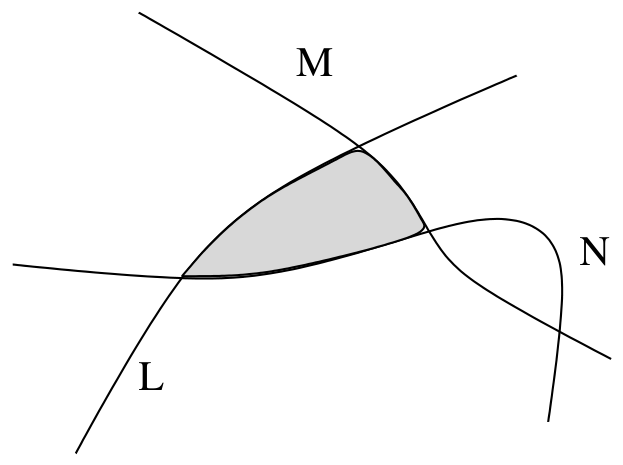
\includegraphics[width=0.4\textwidth]{fig03-floer-product.png}
\end{center}
% [Tutor Note: $\mu^2$ 的两个输入次序极易写反。本文的约定是 $\mu^2(x,y)$ 中 $x\in HF^*(M,N)$
%   为“较晚”的态射、$y\in HF^*(L,M)$ 为“较早”的态射，故合成顺序是“先 $y$ 后 $x$”；
%   而 $H(\scrA)$ 中的结合合成带着分次符号 $[a]\cdot[b]=(-1)^{|b|}[\mu^2(a,b)]$。
%   本节的三角乘积与 §4.1 的 $A_\infty$ 约定必须一致，核对时以 $(-1)^{|a|}$ 是作用在
%   第一个变元还是第二个变元上为第一要务（链层次关系 $d\mu^2(x,y)=\mu^2(dx,y)\pm\mu^2(x,dy)$
%   的符号随此约定联动）。]

图中表明：给定 $L\cap M$ 与 $M \cap N$ 中的输入交点（假定横截），某个给定输出点（位于 $L\cap N$）的系数由图中所示的一族三角形的计数给出；这里照例有若干保留条件：只计数零维模空间的元素，需在适当的几何假设下保证紧性，并且在原则上可以有无穷多个不同模空间作出贡献时要取 Novikov 系数。

\begin{figure}[ht]
  \centering
  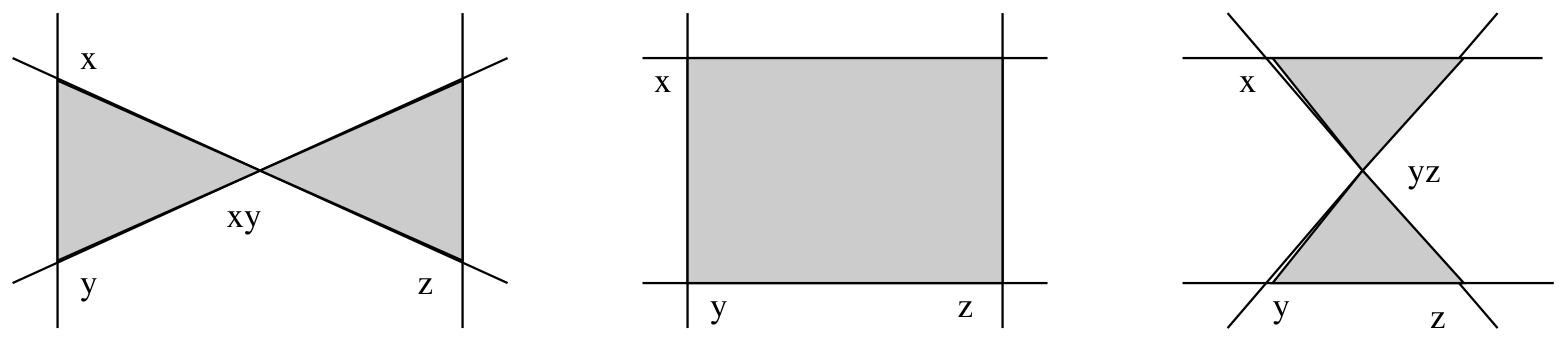
\includegraphics[width=0.78\textwidth]{fig04-triangle-assoc.png}
  \caption{三角乘积在上同调上满足结合律（原文 Figure~3，第 17 页）。\label{Fig:BrokenTriangles}}
\end{figure}

链层次运算之所以能下降到上同调，反映的是如下事实：模去冒泡之后，此类三角形的一维模空间的边界由“在角点处断开”的破裂构型所给出的层组成，而这些层在某个固定输出交点处的系数正是 $\mu^2(d(x),y)$、$\mu^2(x,d(y))$ 与 $d\mu^2(x,y)$ 的系数，其中 $d$ 是 Floer 微分。类似地，四边形的 1 维模空间可以如图 \ref{Fig:BrokenTriangles} 所示那样破裂，这表明三角乘积在上同调上结合：若所有输入都是 Floer 闭链，即 $d(\cdot) = 0$，则只有那两个“拼接三角形”的图形给出该一维模空间边界上非平凡的层，而它们分别对应 $\mu^2(x,\mu^2(y,z))$ 与 $\mu^2(\mu^2(x,y),z)$ 中右上交点的系数。

由此可知，对单个拉格朗日子流形 $L$，$HF^*(L,L)$ 自然地构成一个环，而且还是有单位元的环。环 $HF^*(L,L)$ 具有 Poincaré 对偶，它来自把全纯条带两侧的边界条件互换。事实上，存在迹 $\tr: HF^{n}(L,L) \rightarrow \bK$，它与三角乘积一起给出非退化配对
\[
HF^*(K,L) \otimes HF^{n-*}(L,K) \stackrel{\tr}{\longrightarrow} \bK.
\]
% [Tutor Note: 这里的 Poincaré 对偶就是“交换条带两端的边界条件”：$\tr$ 只在最高次
%   $HF^{n}(L,L)$ 上取值，配对 $HF^*(K,L)\otimes HF^{n-*}(L,K)\to\bK$ 把 $(x,y)$ 送到
%   $\tr(\mu^2(x,y))$。注意次数是 $n-*$ 而不是 $n+*$，且配对两侧 $K,L$ 的次序互换；
%   若定向或分次约定取反，$\tr$ 可能整体差一个 $(-1)^{n(n+1)/2}$，这与 §1 中相交数
%   公式的符号因子是同一个来源。]

下面的命题本质上属于 Oh \cite{Oh:Thomas}（与环结构的相容性在 \cite{Buhovski:ring} 中被明确写出），另见 \cite{Albers,BiranCornea}。它给出了本学科中的一个关键计算工具。

\begin{Proposition}\label{Lem:Oh}
存在谱序列 $H^*(L;\Lambda) \Rightarrow HF^*(L,L)$，它与普通上同调与 Floer 上同调中的环结构相容。
\end{Proposition}

\begin{proof}[证明概要]
固定 Morse 函数 $f: L \rightarrow \bR$。如定理 \ref{Lem:Floer} 中那样，对适当的 $J$，Morse 流线可用来定义 Floer 轨道。该谱序列来自按作用量对 Floer 微分作过滤，使得所有低能量解都来自 Morse 轨道。在作用量与指标相关的单调情形，该谱序列来自把 Floer 微分写成和式 $\partial_0 + \partial_1 + \cdots + \partial_k$，其中 $\partial_0$ 是 $C^*_{Morse}(L)$ 中的 Morse 微分，而 $\partial_i$ 的次数为 $1-iN_L$，$N_L$ 是 $L$ 的极小 Maslov 数。更形象地说，Floer 上同调有一个 Morse–Bott（或“珠串”）模型 \cite{BiranCornea}，其中 Floer 微分计数被 $L$ 上的全纯圆盘打断的 $f$ 的梯度线，参见图 \ref{Fig:PearlyGradient}，而 $\partial_i$ 所计数的构型中圆盘的总 Maslov 指标为 $iN_L$。Morse 乘积计数流线构成的 $Y$-树，这可以推广到珠串构成的 $Y$-形图，由此给出谱序列与环结构的相容性。
\end{proof}
% [Tutor Note: 谱序列的过滤是“按作用量”而不是“按次数”：低能量解只剩 Morse 流线，
%   于是 $E_1$ 页为 $H^*(L;\Lambda)$，微分逐级修正全纯圆盘的贡献。单调情形下
%   能量与指标相关，才可以把 $\partial$ 按圆盘总 Maslov 指标 $iN_L$ 拆成
%   $\partial_0+\partial_1+\cdots$，且 $\deg\partial_i=1-iN_L$；若能量—指标不相关，
%   “按作用量过滤”给出的只是收敛的滤过而非按次数的直和分解。收敛方向是
%   $H^*(L)\Rightarrow HF^*(L,L)$，核对时勿写反。]

\begin{figure}[ht]
  \centering
  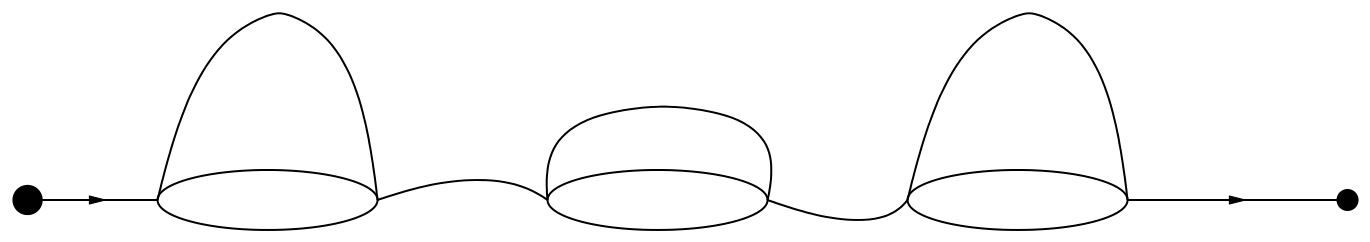
\includegraphics[width=0.68\textwidth]{fig05-pearly.png}
  \caption{Morse–Bott（或“珠串”型）Floer 轨道（原文 Figure~4，第 18 页）。\label{Fig:PearlyGradient}}
\end{figure}

\begin{Example}
环 $HF^*(L,L)$ \emph{并不}总是斜交换的。取 $L = S^1_{eq} \subset \bP^1$；则 $HF^*(L,L) \cong \bC[x]/(x^2=1)$，其中 $|x|=1$ 是最高次生成元，且 $\mu^2(x,x)=1_L$。取珠串模型，该乘积由圆盘 $(D^2, \partial D^2) \rightarrow (\bP^1, S^1_{eq})$ 输出处的取值来定义，这些圆盘带有两个输入标记点，它们是赤道上的固定一般位置点。三个边界标记点有固定的循环次序，由此产生两种可能：若像圆盘是上半球面，取值扫过 $S^1_{eq}$ 上的一条链；若像圆盘是下半球面，则扫过补链。两者合起来构成 $L$ 的基本类。
\end{Example}

\begin{Example} \label{Ex:ToricFibre}
设 $X$ 是单调的，$L\subset X$ 是极小 Maslov 数为 $\mu_L$ 的单调拉格朗日环面。谱序列 $H^*(L) \Rightarrow HF^*(L,L)$ 中的微分 $\partial_1$ 是映射
\begin{equation} \label{Eqn:ToricDifferential}
H^1(L) \longrightarrow H^{2-\mu_L}(L).
\end{equation}
若 $\mu_L=2$ 且该映射非零，则 $H^0(L)$ 中的单位元成为边界，从而在 $HF^*(L,L)$ 中消失，这意味着后者恒为零。若 \eqref{Eqn:ToricDifferential} 为零，则 $H^1(L) \subset \ker(\partial_1)$；由于该核是子环，故 $H^*(L) \subset \ker(\partial_1)$ 且 $\partial_1 \equiv 0$。又因高阶 $\partial_i$ 的次数为 $1-2i \leq -2$，同样的论证表明 $H^1(L)$（从而 $H^*(L)$）位于每个 $\partial_i$ 的核中，这说明谱序列退化。因此，若 $L\subset X$ 是\emph{可移开的}单调环面（例如 $\bC^n$ 中的一个），则由 $HF(L,L)=0$ 可得 $\mu_L = 2$。
\end{Example}

存在一个范畴 Don$(X)$，即 Donaldson 范畴，其对象是（无障碍的）拉格朗日子流形，态射是 Floer 上同调群。合成由全纯三角乘积给出。若 $X$ 是单调的，则该范畴分解为彼此正交的子范畴
\begin{equation} \label{Eqn:DonSplits}
\mathrm{Don}(X) = \bigoplus_{\lambda} \mathrm{Don}(X;\lambda)
\end{equation}
其中 $\lambda$ 取遍 $\frak{m}_0(L)$ 的所有可能值，因为只有当 $\frak{m}_0(L) = \frak{m}_0(L')$ 时，$HF^*(L,L')$ 才对一对拉格朗日有良好定义。由于 $\frak{m}_0(L)$ 计数 Maslov 指标 2 的圆盘，若 $X$ 的极小 Chern 数 $>1$，则任何单连通的拉格朗日都必然落在 Don$(X;0)$ 中。
% [Tutor Note: 分解 \eqref{Eqn:DonSplits} 的依据是 $\frak{m}_0(L)$ 只依赖于单个拉格朗日；
%   两个分支 $\lambda\neq\lambda'$ 之间没有非零态射，故是“正交”直和而非普通直和。
%   注意 $\frak{m}_0(L)$ 是 Novikov 域中的数（计数带面积的 Maslov 2 圆盘），
%   因此分解的指标集 $\lambda$ 是连续取值的；这与按拓扑不变量进行的离散分解不同。]

\subsubsection{模结构}\label{Subsec:ModuleStructures}

Floer 上同调 $HF^*(L, L')$ 是有单位元环 $HF^*(L,L)$ 上的右模。此外还有量子上同调作用的模结构：对任何（可定向的）拉格朗日 $L$，存在有单位元的环同态
\begin{equation} \label{Eqn:ClosedOpen}
\mathcal{CO}^0: QH^*(X) \longrightarrow HF^*(L,L)
\end{equation}
称为（闭-开弦映射的长度零部分）。它通过计数以 $L$ 为边界的全纯圆盘来定义：圆盘带一个内部输入标记点，该点被约束在 $X$ 中代表某个 $QH^*$-生成元的闭链上；另有一个边界标记点，我们在该点取值以定义输出的 Floer 类。$QH^*(X)$ 是交换的，且 $\mathcal{CO}^0$ 的像落在 $HF^*(L,L)$ 的中心。

\begin{Example}
$\bC\bP^n$ 的量子上同调为 $\Lambda[x]/(x^{n+1}=1)$，其中 $|x|=2$。设 $L\subset \bC\bP^n$ 是拉格朗日子流形。若 $HF^*(L,L)$ 有良好定义，则由 $x$ 在 $HF^*(L,L)$ 中的像可逆可知，后者必须是 2-周期的。
\end{Example}

Auroux、Kontsevich 与 Seidel 的一个美妙观察 \cite{Auroux} 是：在单调情形下、并避开特征 2，映射 \eqref{Eqn:ClosedOpen} 把 $c_1(X) \mapsto \frak{m}_0(L) e_L$，这意味着 \eqref{Eqn:DonSplits} 中出现的值 $\lambda$ 恰好是自同态 $\ast c_1(X)$ 作用在 $QH^*(X)$ 上的特征值。简短讨论见注 \ref{Rem:StarC1}。
% [Tutor Note: $\frak{m}_0(L)$ 与量子上同调的联系是本节的深层要点：闭-开弦映射把
%   $QH^*(X)$（由 $X$ 的 Gromov–Witten 理论决定）送到 $HF^*(L,L)$，而 $c_1(X)$ 的像
%   正是 “Maslov 2 圆盘计数” $\frak{m}_0(L)$ 乘以单位元 $e_L$。因此 $\frak{m}_0(L)$
%   不是自由参数，而必须等于 $\ast c_1(X)$ 在 $QH^*(X)$ 上的某个特征值——
%   这正是 \eqref{Eqn:DonSplits} 中 $\lambda$ 的取值有限（离散）的原因。
%   易错点：$c_1\mapsto\frak{m}_0(L)e_L$ 成立需要“单调 + 特征 $\neq 2$”；
%   $e_L$ 是 $HF^*(L,L)$ 的单位元，而 $\frak{m}_0(L)\in\Lambda$ 属系数域。]

\subsubsection{正合三角\label{Subsec:ExactTriDon}}

暂且这样定义：三个拉格朗日子流形与态射
\[
\xymatrix{ L \ar^{a}[r] & L' \ar^{b}[r] & \ar@/^1.5pc/[ll]_{[1]} L''}
\]
在 Don$(X)$ 中构成一个\emph{正合三角}，如果对任意另一个拉格朗日 $K$，与给定态射（Floer 闭链）作复合诱导出 Floer 上同调群的长正合列
\[
\cdots  \rightarrow HF^i(K,L) \stackrel{a}{\longrightarrow} HF^i(K,L')\stackrel{b}{\longrightarrow} HF^i(K,L'') \rightarrow HF^{i+1}(K,L) \rightarrow \cdots.
\]
也许令人惊讶的是，正合三角确实存在：
% [Tutor Note: “正合三角”在这里是由 Yoneda 型条件定义的：对每个测试对象 $K$，
%   $HF^*(K,\cdot)$ 把三角 $L\to L'\to L''$ 变成长正合列；并非三角本身在链层次
%   正合。弧上的 $[1]$ 表示映射锥的平移，方向（逆时针）也是约定的一部分，
%   画反会改变三角的定向。]

\hspace{1em} $\bullet$ 若 $L \pitchfork L' = \{p\}$ 横截相交于唯一一点，且 $L'' = L\# L'$ 是 Lagrange 手术 \cite{Polterovich}（拓扑上即连通和：把二重点的邻域 $\bR^n \cup i\bR^n$ 换成一个拉格朗日 1-柄 $S^{n-1} \times \bR$），则 \cite{BiranCornea2, FO3} 存在正合三角 $L \stackrel{p}{\longrightarrow} L' \longrightarrow L''$。在图 \ref{Fig:SurgeryTriangle} 中，直的拉格朗日 $L, L'$ 的交点从左至右被消解；虚线弧是第三个拉格朗日 $K$；可以看到右图中有两个全纯圆盘对复形 $CF^*(K, L\#L')$ 作出贡献，一个来自复形 $CF^*(K,L)$，另一个来自与 $p$ 的乘法（把该点视为映射 $CF(K,L) \rightarrow CF(K,L')$），这示意性地给出拟同构
\[
CF(K,L\#L') \stackrel{\sim}{\longrightarrow} \left( CF(K,L) \oplus CF(K,L'), \left(\begin{array}{cc} \partial_L & 0 \\ \mu^2(p,\cdot) & \partial_{L'} \end{array} \right)\right)
\]
（在更高维情形，从刚性全纯三角形的集合到以 $K$ 与 $L\#L'$ 为边界的刚性圆盘的相应单射并非平凡）。
% [Tutor Note: 右端矩阵微分的非对角项 $\mu^2(p,\cdot)$ 是符号与次序的双重易错点：
%   它把 $CF(K,L)$ 送到 $CF(K,L')$，其中 $p\in CF(L,L')=HF^*(L,L')$ 充当“较晚”的
%   变元；若把 $p$ 放进第二个变元或漏掉分次符号 $(-1)^{|p|+1}$ 型因子，
%   $\partial^2=0$ 会失效，且手术三角的定向随之出错。对角块是 $\partial_L,\partial_{L'}$，
%   次序对应直和分解 $CF(K,L)\oplus CF(K,L')$，不要与上三角/下三角混淆。]

\begin{figure}[ht]
  \centering
  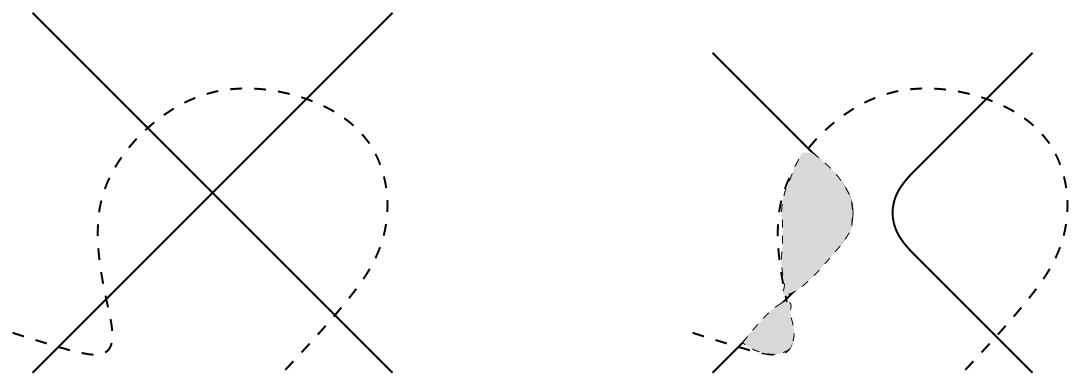
\includegraphics[width=0.5\textwidth]{fig06-surgery-tri.png}
  \caption{走向手术正合三角（原文 Figure~5，第 20 页）。\label{Fig:SurgeryTriangle}}
\end{figure}

% 原文此处有 \newcommand{\ev}{\mathrm{ev}}；本译稿的导言区已定义 \ev，故略去以免重复定义报错。

\hspace{1em} $\bullet$ 若 $V\cong S^n \subset X$ 是（单调或恰当的）拉格朗日球面，$\tau_V$ 表示沿 $V$ 的 Dehn 扭转，则 \cite{Seidel:LES} 在 Don$(X)$ 的加法扩张中存在正合三角 $L \stackrel{\phi}{\longrightarrow} \tau_V(L) \rightarrow HF^*(V,L)\otimes V$；所谓加法扩张，就是我们形式地允许对象的直和，或等价地允许拉格朗日与分次向量空间作张量积。固定任意另一个拉格朗日 $K$。首先把 $K \cap \tau_V(L)$ 的交点与 $K \cap L$ 的点（我们假定这些点位于 $\tau_V$ 的支集之外）等同起来，再对 $V \cap L$ 的每个点附加一份 $K \cap V$，因为每当 $L$ 与 $V$ 相交，$\tau_V$ 就把 $L$ 绕 $V$ 缠绕一圈。于是在向量空间层次上
$CF(K,\tau_V(L))  = CF(K,L) \oplus (CF(V,L)\otimes CF(K,V))$。态射 $\phi$ 计数 $D^2\backslash \{-1\}$ 上 Lefschetz 纤维化的截面，该纤维化在 $0$ 处有一个临界点（消没圈 $V$ 在那里被收缩为一点），边界条件为 $L, \tau_V(L)$。所需的同伦
\begin{equation} \label{Eqn:Nullhtpy}
\kappa: CF(V,L) \rightarrow CF(V,\tau_V(L)), \quad \partial \kappa \pm \kappa \partial + \mu^2(\phi, \cdot) = 0
\end{equation}
由如图 \ref{Fig:LESnullhtpy} 的一族单参数 Lefschetz 纤维化得到，并由此给出长正合列。左端看到的是复合 $\mu^2(\phi,\cdot)$；图中最右的纤维化没有刚性截面，因为模型 Lefschetz 纤维化 $\bC^{n+1} \rightarrow \bC$ 在以已经冒泡的消没圈 $V$ 为边界条件时\emph{没有}这样的截面——模型的所有截面模空间的虚维数都是奇数。因此，若 $\kappa$ 计数整个族中的刚性曲线，就得到 \eqref{Eqn:Nullhtpy}。把 $\kappa$ 视为映射 $CF(V,L)\otimes V \rightarrow \tau_V(L)$，并令 $\ev: CF(V,L) \otimes V \rightarrow L$ 为自然的取值映射，则 \eqref{Eqn:Nullhtpy} 表明 $\mu^2(\phi,\ev)$ 经 $\kappa$ 零伦，从而按需把 Cone$(\ev)$ 与 $\tau_V(L)$ 等同起来。
% [Tutor Note: \eqref{Eqn:Nullhtpy} 里的 $\pm$ 号取决于定向与分次约定，原文有意保留
%   未定；核对时应把 $\kappa$ 的度数与 $\mu^2(\phi,\cdot)$ 的度数一起检查，才能确定
%   是 $+$ 还是 $-$。几何上，$\kappa$ 是一族 Lefschetz 纤维化的刚性截面计数：
%   左端的纤维化给出 $\mu^2(\phi,\cdot)$，右端因模型纤维化的截面模空间虚维数为奇而
%   无刚性截面，于是整族的计数恰好给出零伦。另有一步易漏：把 $\kappa$ 视为
%   $CF(V,L)\otimes V\to\tau_V(L)$ 时要用取值映射 $\ev$ 与 $\mu^2$ 的配对。]

\begin{figure}[ht]
  \centering
  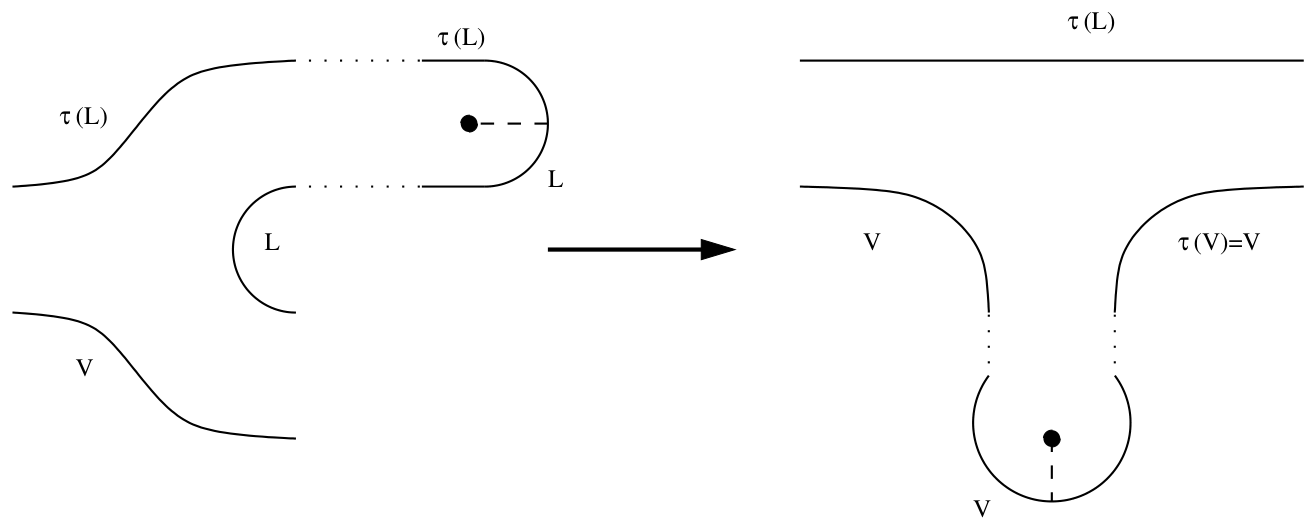
\includegraphics[width=0.7\textwidth]{fig07-les-nullhtpy.png}
  \caption{走向 Dehn 扭转正合三角（原文 Figure~6，第 21 页）。\label{Fig:LESnullhtpy}}
\end{figure}

\subsubsection{来自对应的函子}\label{Sec:Quilt}

记 Don$^{\#}(Y)$ 为 $Y$ 的广义拉格朗日子流形范畴，其对象是拉格朗日对应的序列
\[
\{pt\} \stackrel{L_0}{\longrightarrow} Y_0 \stackrel{L_{01}}{\longrightarrow} \cdots \stackrel{L_{k-1,k}}{\longrightarrow} Y_k = Y
\]
其中 $L_{i,i+1} \subset Y_i^- \times Y_{i+1}$ 是拉格朗日子流形。这里 $(Y,\omega_Y)^- = (Y, -\omega_Y)$。Wehrheim 与 Woodward \cite{WW1, WW2} 把 Floer 上同调（本质上是形式地）推广到广义拉格朗日对。例如给定 $L \subset X$、$K\subset Y$ 与 $\Gamma \subset Y^- \times X$，$HF(L, (\{pt\} \stackrel{K}{\longrightarrow} Y \stackrel{\Gamma}{\longrightarrow} X))$ 按定义就是在 $Y^- \times X$ 中计算的 $HF(K \times L, \Gamma)$。Floer 乘积到广义拉格朗日的推广更为复杂，涉及对“quilt 化”黎曼曲面的计数（这类曲面的内部接缝标以拉格朗日边界条件）。设 $(X,\omega_X)$ 与 $(Y,\omega_Y)$ 是辛流形，$\Gamma \subset X^-\times Y$ 是拉格朗日对应，其中 $X^-$ 表示 $(X,-\omega)$。在强单调性假设下，$\Gamma$ 诱导函子
\[
\Phi_{\Gamma}: \mathrm{Don}(X) \longrightarrow \mathrm{Don}^{\#}(Y),  \qquad  \Phi_{\Gamma}: L \, \mapsto \,  \left( \{pt\} \stackrel{L}{\longrightarrow} X \stackrel{\Gamma}{\longrightarrow} Y\right)
\]
它在对象上按所示拼接方式作用。Wehrheim 与 Woodward 的一个重要而困难的定理是：若几何复合
\[
\Gamma \circ L \ = \ \left\{ u \in Y \ \big| \ (x,u) \in \Gamma \ \mathrm{for \ some} \ x\in L\, \right\}
\]
是嵌入的拉格朗日子流形，则 $\Phi_{\Gamma}(L)$ 与 $\Gamma\circ L$ 在 Don$^{\#}(Y)$ 中同构（特别地，形式复合与通常 Donaldson 范畴中的某个对象同构）。利用 quilt 理论，可以构造一个底层的函子
\begin{equation} \label{Eqn:QuiltFunctor}
\Phi: \mathrm{Don}(X^- \times Y) \longrightarrow \mathrm{Fun}(\mathrm{Don}(X), \mathrm{Don}^{\#}(Y))
\end{equation}
其中 $\Phi: \Gamma \mapsto \Phi_{\Gamma}$。特别地，若 $HF(\Gamma,\Gamma) = 0$（在 $X^-\times Y$ 中计算），则 $\Phi_{\Gamma}$ 是零函子；而若 $\Phi_{\Gamma}(L) \neq 0$，则 $\Gamma \neq 0$。
% [Tutor Note: 函子 \eqref{Eqn:QuiltFunctor} 的“形式化”之处要分清两个层次：
%   对象上只是把对应 $\Gamma$ 拼接到 $L$ 后面（符号记法），真正的函子性依赖 quilt
%   模空间的计数——即带内部接缝（标以拉格朗日边界条件）的黎曼曲面的全纯映射。
%   Wehrheim–Woodward 定理的实质是：当几何复合 $\Gamma\circ L$ 是嵌入子流形时，
%   形式复合 $\Phi_{\Gamma}(L)$ 与它在 $\mathrm{Don}^{\#}(Y)$ 中同构，从而“形式”范畴
%   并不比几何范畴更病态。注意 $\mathrm{Don}^{\#}$ 的对象是序列而非单个流形。]

\begin{Example} \label{Ex:Corr}
参见 \cite{WW2}。记 $S^3 \subset \bC^2$ 为单位球面。Hopf 映射 $h: S^3 \rightarrow S^2$ 满足 $(\omega_{\st})|_{S^3} = h^*(\omega_{\operatorname{FS}})$。复合 $(\mathrm{antipodal})\circ h$ 的图定义了 $B^4(r) \times \bP^1$ 的拉格朗日子流形（对任意 $r>1$），从而得到带单调辛形式的拉格朗日子流形 $\Gamma=S^3 \subset \bP^2 \times \bP^1$。把 $\Gamma$ 视为从 $\mathrm{Don}(\bP^1)$ 到 $\mathrm{Don}^{\#}(\bP^2)$ 的函子。像 $\Phi_{\Gamma}(S^1_{eq})$ 拟同构于 $\bP^2$ 中的 Clifford 环面。由例 \ref{Ex:ToricFibre} 可知它具有非平凡的自 Floer 上同调，这意味着 $HF(\Gamma,\Gamma) \neq 0$。
\end{Example}

初看之下，过渡到 Don$^{\#}(Y)$ 稍显吓人：其定义涉及中间辛流形的任意序列，似乎难以驾驭。然而，给定有限个拉格朗日 $\{L_i\} \subset Y$ 及相应的代数 $A = \oplus_{i,j} HF^*(L_i, L_j)$，存在一个函子 Don$^{\#}(Y) \rightarrow \mathrm{mod}$-$(A)$，它把任一广义拉格朗日送到它与诸 $L_i$ 的 Floer 上同调之直和；这使人得以把非交换代数的工具用于这个扩张范畴。
% [Tutor Note: 这里的 $A=\oplus_{i,j}HF^*(L_i,L_j)$ 只记录了对象之间的 Floer 群，
%   还不含高阶运算；函子 $\mathrm{Don}^{\#}(Y)\to\mathrm{mod}$-$A$ 是“取与诸 $L_i$
%   的 Floer 上同调”的直和，属于 Yoneda 型构造。它在观念上把几何范畴嵌入
%   非交换代数，但丢失了 $A_\infty$ 的高阶信息——这正是 §4 要补上的结构。]

\subsection{应用 II}

我们简要说明迄今引入的代数结构如何扩大理论的适用范围；这些例子取自 \cite{Buhovsky} 与 \cite{Smith:HFQuadrics}。

\subsubsection{附近的拉格朗日}

设 $L \subset T^*S^{2k+1}$ 是恰当拉格朗日，且 $H_1(L;\bZ) = 0$。我们断言 $H^*(L) \cong H^*(S^{2k+1})$。如例 \ref{Ex:Corr} 那样，Hopf 映射
\[
\bC^{k+1}\backslash \{0\} \supset S^{2k+1} \stackrel{h}{\longrightarrow} \bP^k
\]
由取射影化给出，其性质是 $h^*\omega_{\operatorname{FS}} = (\omega_{\st})|_{S^{2k+1}}$。因此，取图可得到拉格朗日嵌入 $S^{2k+1} \subset \bC^{k+1} \times (\bP^k)^-$。如有必要把 $L\subset T^*S^{2k+1}$ 缩放使其靠近零截面，则 $L$ 也嵌入这一乘积中。由假设 $H_1(L;\bZ) = 0$，该嵌入是单调的，因此 $HF(L,L)$ 有良好定义，在乘积 $\bC^{k+1} \times (\bP^k)^-$ 中计算。由于可在第一个因子上作平移，它显然可以被移开自身，故 $HF(L,L)=0$。

现在考虑 Oh 谱序列，即命题 \ref{Lem:Oh}。$L$ 在 $T^*S^{2k+1}$ 中的 Maslov 类为零，但在 $\bC^{k+1} \times (\bP^k)^-$ 中的极小 Maslov 数为 $2k+2$。这意味着 Oh 谱序列中唯一非平凡的微分形如
\[
H^{i+2k+1}(L) \rightarrow H^i(L) \rightarrow H^{i-2k-1}(L) \qquad \forall \ 0 \leq i \leq 2k+1.
\]
所需结论随即得到。

\subsubsection{映射类群}

设 $S$ 是亏格 2 的闭曲面，$p
\in S$，而 $\scrM(S)$ 是把边界环路送到 $-I$ 的表示 $\pi_1(S\backslash \{p\})$ 到 $SU(2)$ 的共轭类的模空间。它是辛的，因为它是秩二丛 $E \rightarrow S$ 上联络的无穷维空间的商，而后者带有自然辛形式 $\omega(a,b) = \int_S \tr(a \wedge b)$，其中 $a,b \in \Omega^1(S;\End(E))$。固定 $p$ 不动的 $S$ 的微分同胚构成映射类群 $\Gamma(S,p)$，它辛地作用在 $\scrM(S)$ 上；我们断言，对任意 $\phi \in \Gamma(S,p)$，都有 $HF^*(\phi) \neq \{0\}$。

证明的核心是如下归纳论证。同调本质的简单闭曲线 $\gamma \subset S$ 通过取沿 $\gamma$ 和乐平凡的联络，定义了拉格朗日 3-球面 $SU(2) \cong L_\gamma \subset \scrM(S)$。Dehn 扭转 $\tau_\gamma \in \Gamma(S,p)$ 通过高维 Dehn 扭转 $\tau_{L_{\gamma}}$ 作用在 $\scrM(S)$ 上。空间 $\scrM(S)$ 是单调的，极小 Chern 数为 2，且 Spec$(\ast c_1: QH^*(\scrM(S)) \rightarrow QH^*(\scrM(S)))$ 为 $\{0, \pm 4i\}$。存在正合三角
\begin{equation} \label{Eqn:InductiveTriangle}
\xymatrix{ HF^*(\phi) \ar[r] & HF^*(\tau_{L_\gamma} \circ \phi)  \ar[r] & \ar@/^1.5pc/[ll]^{[1]} HF^*(L_{\gamma}, \phi(L_{\gamma}))}
\end{equation}
对任意 $\phi \in \Gamma(S,p)$ 与本质曲线 $\gamma \subset S$ 成立。考虑特征值 $4i$ 的相应广义特征空间所构成的正合三角。由于 $c_1 \mapsto \frak{m}_0(L_{\gamma}) \in HF^*(L_{\gamma}, L_{\gamma}) = A$，且 $L_{\gamma}$ 的极小 Maslov 数 $>2$，故 $c_1$ 在 $A$ 上平凡地作用，从而在 $A$-模 $HF^*(L_{\gamma}, \phi(L_{\gamma}))$ 上平凡地作用。由此可知，特征值 $4i$ 的 $\ast c_1$-广义特征空间在复合 $\tau_{L_{\gamma}}$ 下不变；类似的论证表明它在复合逆 Dehn 扭转下也不变。由于这类扭转生成映射类群，归纳地只需证明相应特征空间对 $HF^*(\id)\cong QH^*(\scrM(S))$ 非零。Newstead 的一个定理 \cite{Newstead} 把 $\scrM(S)$ 等同于 $\bP^5$ 中两个二次超曲面的交，由此 $QH^*$ 的计算是直接的 \cite{SKD}：$4i$-广义特征空间的秩为 1。

一个推论是：若 $Y \rightarrow S^1$ 是由亏格 2 曲线纤维化的任意 3-流形，则 $\pi_1(Y)$ 容许非阿贝尔的 $SO(3)$-表示。
% [Tutor Note: 正合三角 \eqref{Eqn:InductiveTriangle} 的直观是：沿本质曲线 $\gamma$ 作
%   高维 Dehn 扭转 $\tau_{L_\gamma}$ 不改变 $\ast c_1$-广义特征空间；而这类扭转生成
%   映射类群，故只须验证恒等映射这一情形。易错点：$\frak{m}_0(L_\gamma)$ 在
%   $HF^*(L_\gamma,L_\gamma)=A$ 中是单位元的倍数，因此 $c_1$ 在 $A$ 上的作用是
%   “乘以常数”，它在 $A$-模上仍是常数倍——这一步用到了 $L_\gamma$ 的极小 Maslov
%   数 $>2$（否则 $\frak{m}_0$ 不再只由单位元贡献）。]

\subsection{不足}\label{Subsec:Shortcoming}

下述情形经常出现：给定的辛流形 $X$ 含有某个有限的“区分”拉格朗日子流形族，人们期待通过迭代地取态射的锥（例如通过 Lagrange 手术，或取 Dehn 扭转下的像）来生成所有拉格朗日。这有限族拉格朗日 $\{L_i\}$ 定义一个环
\[
A = \oplus_{i,j} HF^*(L_i, L_j)
\]
而任何其他拉格朗日 $K$ 定义一个右 $A$-模
\[
Y_K = \oplus_i HF^*(L_i, K).
\]
现在给定两个拉格朗日 $K, K'$，可以考虑两个显然的群：一个是几何地定义的 Floer 上同调 $HF^*(K,K')$，另一个是代数地定义的态射群 $\Ext_{A-mod}^*(Y_K, Y_{K'})$。就目前发展出的结构而言，即便 $\{L_i\}$ “应当生成”的直觉是正确的，这两个群通常也不会相同。

\begin{figure}[ht]
  \centering
  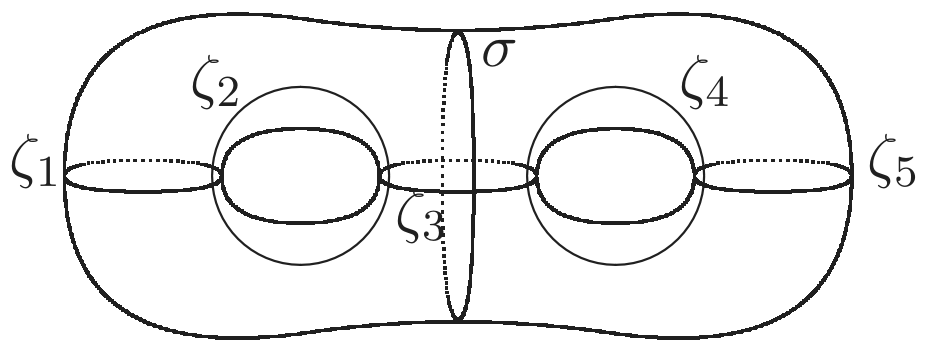
\includegraphics[width=0.45\textwidth]{fig08-genus2.png}
  \caption{亏格 2 曲面；图中标出曲线 $\zeta_1$、$\zeta_2$、$\zeta_3$、$\zeta_4$、$\zeta_5$ 与 $\sigma$（原文 Figure~7，第 23 页）。\label{Fig:genus2pencil}}
\end{figure}

\begin{Example}
考虑亏格 2 曲面。曲线 $\zeta_i$ 生成所有简单闭曲线，意思是任何同伦本质的曲线必与某个 $\zeta_i$ 有非平凡的几何相交数；且 Dehn 扭转 $\tau_{\zeta_j}$ 生成映射类群\footnote{由命题 \ref{Prop:SpheresGenerate} 可知，曲线 $\zeta_i$ 分裂生成 Fukaya 范畴。}。在环 $A = \oplus_{i,j} HF^*(\zeta_i, \zeta_j)$ 上，由曲线 $\sigma$ 定义的模 $Y_{\sigma}$ 同构于 $\zeta_3$ 上的单模与其平移之和 $\hat{Y}_{\sigma} = S_{\zeta_3} \oplus S_{\zeta_3}[1]$，这本质上是因为图中没有非常值的全纯月牙或三角形。然而，$S_{\zeta_3} \oplus S_{\zeta_3}[1]$ 的自同态代数是矩阵代数，特别地 Ext$_{A-\mathrm{mod}}(\hat{Y}_{\sigma}, \hat{Y}_{\sigma}) \not \cong HF^*(\sigma,\sigma) = H^*(S^1)$。
\end{Example}

问题在于：$A$ 并不只是一个环；把它仅仅当作环，就忽略了重要的结构——我们下面引入该结构。
% [Tutor Note: 本例是 §3.8 的核心：$\Ext_A$ 与 $HF^*$ 的差异不是技术性误差，而是
%   因为 $A$ 缺少 $A_\infty$ 的高阶运算。$Y_\sigma\cong S_{\zeta_3}\oplus S_{\zeta_3}[1]$
%   之所以成立，是由于图中没有非常值的全纯月牙/三角形；而矩阵代数的自同态群
%   比 $HF^*(\sigma,\sigma)=H^*(S^1)$ 大，说明“只记住环 $A$”会丢失信息。
%   这是下一节引入 Fukaya 范畴（$A_\infty$-结构）的直接动机。]

\begin{Notes}
关于 Floer（与量子）上同调的基础，参见 \cite{Floer, Oh, AudinDamian, McD-S2}。关于代数结构，参见 \cite{BiranCornea, FO3, WW2, RitterSmith}，以及 Seidel 的许多论文，例如 \cite{Seidel:graded, Seidel:MCG, Seidel:LES, Seidel:twist}。
\end{Notes}
